% \usetheme[progressbar=frametitle]{metropolis}
\usepackage{appendixnumberbeamer}
\usepackage[utf8]{vietnam}
\usepackage[utf8]{inputenc}
\usepackage[vietnamese]{babel}
\usepackage[T1]{fontenc}
%\renewcommand\sfdefault{cmbr}
\usepackage{booktabs}
\usepackage[scale=2]{ccicons}
\usepackage{ragged2e}
\apptocmd{\frame}{}{\justifying}{}
\usepackage{pgfplots}
\usepgfplotslibrary{dateplot}
\usepackage[upright]{fourier}
\usepackage{tikz}



\usetikzlibrary{matrix,arrows,decorations.pathmorphing}


\definecolor{rosy}{RGB}{247, 215, 148}
\definecolor{summer}{RGB}{245, 205, 121}
\definecolor{beige}{RGB}{253, 227, 167}
\definecolor{sblack}{RGB}{64, 64, 64}
\setbeamercolor{frametitle}{bg=rosy,%bg=beige,
fg=sblack}

\usepackage{hyperref}
\hypersetup{
    colorlinks=true,
    linktoc=all,
    linkcolor=black,
}
\usepackage{relsize}
\usepackage{textpos}
\addtobeamertemplate{frametitle}{}{%
\begin{textblock*}{100mm}(\textwidth,-1.05cm)
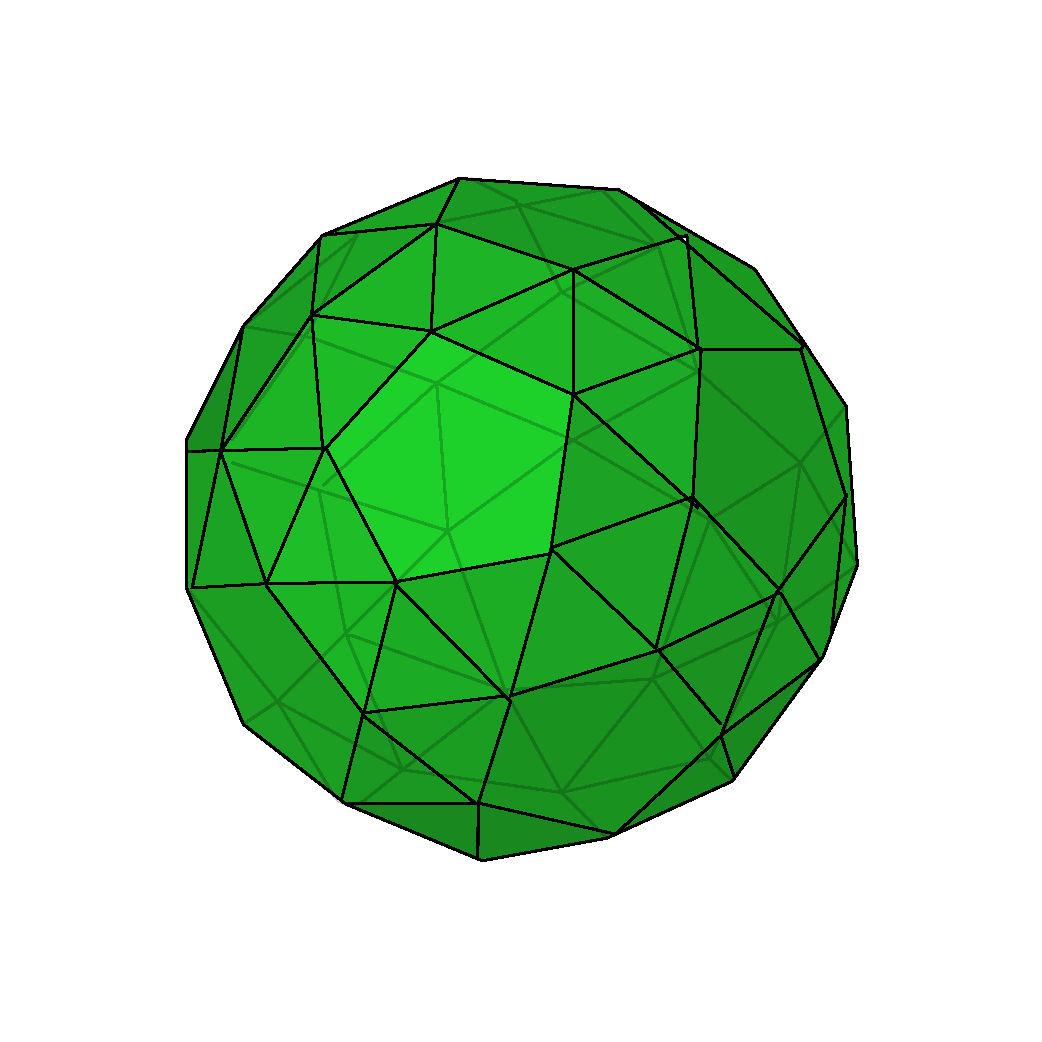
\includegraphics[height=1cm,width=1cm,keepaspectratio]{logo.pdf}
\end{textblock*}}

\usepackage{xspace}

\setbeamerfont{page number in head/foot}{size=\tiny}
\setbeamercolor{footline}{fg=gray}
\setbeamertemplate{frame footer}{PiMA 2019: The Mathematics of Deep Learning}

% \newcommand{\themename}{\textbf{\textsc{metropolis}}\xspace}
\usepackage{cmbright}
